% timetags
%
\documentclass[10pt,dvips]{article}
%\documentclass[10pt,twocolumn,dvips]{article}
\usepackage[english]{babel}
\usepackage{epsfig}
%\usepackage{fancyheadings}
%\usepackage[T1]{fontenc}
%\usepackage[latin1]{inputenc}
%\usepackage{twocolumn}
%\usepackage{verbatim,moreverb,doublespace}
%\usepackage{rotate,lscape,dcolumn,array,rotating,latexsym}
%
%\input{epsf}
%
% for somebody (I forget now !)
%\textwidth 175mm
%\textheight 225mm
%\topmargin -4.5mm
%
% for somebody else (I also forget now !)
%\textwidth 6.6in 
%\textheight 239mm
%\topmargin -15mm
%\leftmargin -2.0in
%
% for HPCA (IEEE single-column format)
\textwidth 6.875in
\textheight 8.875in
\topmargin -0.6in
\oddsidemargin 0mm
\evensidemargin 0mm
%
%
\pagestyle{empty}
%
\begin{document}
%\parskip 1mm
\parskip 2mm
%
%
\title{Preserving Dependencies in a Large-Scale Distributed 
Microarchitecture}
%
\author{
A. Khalafi, D. Morano, D.R. Kaeli\\
Northeastern University\\
dmorano, kaeli@ece.neu.edu\\
\and
A.K. Uht\\
University of Rhode Island\\ 
uht@ele.uri.edu
}
% For a paper whose authors are all at the same institution,
% omit the following lines up until the closing ``}''.
% Additional authors and addresses can be added with ``\and'',
% just like the second author.
%
\date{}
%
\maketitle
%
% uncomment the following for page with no page numbers (for IEEE)
%\thispagestyle{empty}
%
%
\begin{abstract}
We discuss a means by which a large distributed and scalable
microarchitecture can be controlled in a distributed way using
{\em time tags}.  Time tags serve as the basic ordering enforcement mechanism
when large numbers of instructions are executing concurrently and
are also spatially distributed on silicon or multi-chip modules.
They enable the management of the architected program order as
it executes.  The design, use and management of time tags will
be discussed.  We also provide simulation data showing how a modestly large
and microarchitecturally distributed machine performs using
the time tag based design approach described.
\end{abstract}
%
%
\section{Introduction}
%
A number of studies into the limits of 
instruction level parallelism (ILP) have
been promising in that they have shown that there is parallelism within
typical programs~\cite{Gon97,Lam92,Uht95}.  
Unfortunately, most of this fine-grained
parallelism spans several basic blocks and the relatively small
instruction fetch windows of existing processor designs cannot span
the program instruction space necessary to begin to exploit this
parallelism.  A large number of instructions need to be fetched
each cycle and executed concurrently in order to expose this ILP.
A fundamental challenge 
is how to find this parallelism and then allow execution to occur
out of order  
while still maintaining the architectural program order that
is required for proper program execution.
We need to find this ILP at runtime; we need to 
enable the hardware to find, schedule,
and otherwise manage possible control and data independent instructions.

A large, distributed, microarchitecture, capable of executing tens or 
hundreds of instructions concurrently
is needed in order to exploit the fine-grained parallelism present 
in sequential programs.
A barrier encountered when realizing a large-scale microarchitectures is the
competition for centralized machine resources.
These resources often include the 
physical register file (including both architectural as well as renaming 
registers), register renaming logic,
and the reorder buffer.  Other resources that are often centralized
in conventional microarchitectures are the execution units, though they
do not present the same challenges for maintaining correct program order
as those resources that are associated with the architected registers
and the dependencies (control, register, and memory) that arise
from the instructions themselves.  The use of centralized resources
greatly hinders the scalability of any microarchitecture implementation. 

We present a microarchitecture that is able to scale to large sizes
through the
elimination of most conventional centralized microarchitectural components.
We are proposing to use time tags to maintain 
and enforce correct program order for all flow dependencies whether
they be registers, memory values, or instruction control-flow predicates.
A description of the general microarchitecture
assumed in this paper is presented in~\cite{Uht01}.  
In this paper
we focus our attention on the design of time tags and their
associated operations.

Section 2 will discuss a basic distributed microarchitecture that
achieves the above goals and how time tags are defined and used
to coordinate its execution flow.  
Section 3 presents a small set of simulation results that demonstrate
the power of using time tags for dependency enforcement. 
Section 4 discusses some of the differences between our envisioned
microarchitecture and existing schemes.
Section 5 summarizes the current contributions.
%
%
\section{Distributed Microarchitecture Using Time Tags}
%
In order to achieve high IPC in single-threaded, branch-dominated 
program codes, many instructions need to be decoded and executed
in parallel.  We desire that the span of instructions that might be
executed in parallel be on the order of at least tens and possibly hundreds
or thousands.  
Unfortunately, having a large numbers of instructions
in flight simultaneously places an enormous burden on access to 
the physical register file 
(or files, if they are partitioned in some way \cite{Jiser00},
the architected register mapping function, and the reorder buffer 
needed for
management of the final committed program order.

The primary features of the miroarchitecture in view for
our purposes are that it can 
be used to implement
any ISA (most importantly the major existing ones) and
is scalable in terms of the numbers of basic building block
components that can be used as well as at the same time provide
constant length buses regardless of machine size.
The primary feature of the microarchitecture that we focus on
is its use of time tags for dependency enforcement but it
has some other unusual features as well.  
The present microarchitecture
is also designed to be able to execute more than one path
of a program simultaneously and also employs execution-time
predication of all instructions that are in flight.
This is predication at the microarchitectural level and not
related to architected predication that is present in
new ISA like iA-64.  Those ISAs that have architecture predication
can also be implemented on this microarchitecture and there would
still be the microarchitectural predication present.
In the subsections below we describe a number of key elements
of the microarchitecture in order to understand where and how
time tags are used.
%
%
\subsection{Active Stations and Execution Window}
%
To address contention problems encountered with centralized
machine resources, we have extended the idea of the reservation
station \cite{Tom67} to provide the basic building block for a distributed
microarchitecture.  
The idea of the reservation station is extended to 
forward execution results to other spatially
separated and distributed reservation stations
rather than looping the results back to a common instruction dispatch
unit
and update logic for the architected register file.  
We also extend the idea
of the reservation station to allow for multiple executions (re-executions)
of the same instruction in the station.  We will keep an 
instruction in the station until it is retired (either committed or 
squashed).  
We call our adaptation of the reservation station an 
{\em Active Station} (AS).  

Rather than lay our Active Stations out in silicon simply next to
the functional units that will execute the instructions 
dispatched to them,
we will lay them out in a two dimensional grid whereby sequentially
dispatched instructions (in program order) are assigned to 
sequential ASes down a column of
the two dimensional grid of ASes.  
Active stations are grouped together (spatially) so that execution resources
can be shared among them.  Some instruction execution functions such
as floating point calculations are too costly in hardware to not
be shared (statistically multiplexed) among several instructions
that may be in flight at the same time.
The execution resource that is associated with a group of active stations
is termed a \textit{Processing Element} (PE).  One or more processing
elements may be associated with each group of active stations.
A group of active stations that share one or more processing elements
is termed a \textit{Sharing Group} (SG).
Since the ASes and PEs that make up a sharing group are close to each
other in silicon, the interconnections between may be more
extensive than that which is possible in the whole of the execution window.
The two dimensional
grid of ASes, along with their interspersed execution units (PEs),
is called the {\em Execution Window}.
This arrangement is shown in Figure \ref{fig:window}.  
Also shown
in the figure is how ASes and PEs are grouped into SGs.
There are four SGs shown, each with six ASes and one PE.
The total height of each column consists of six ASes and there
are two columns of SGs and four columns of ASes.
%
\begin{figure}
\centering
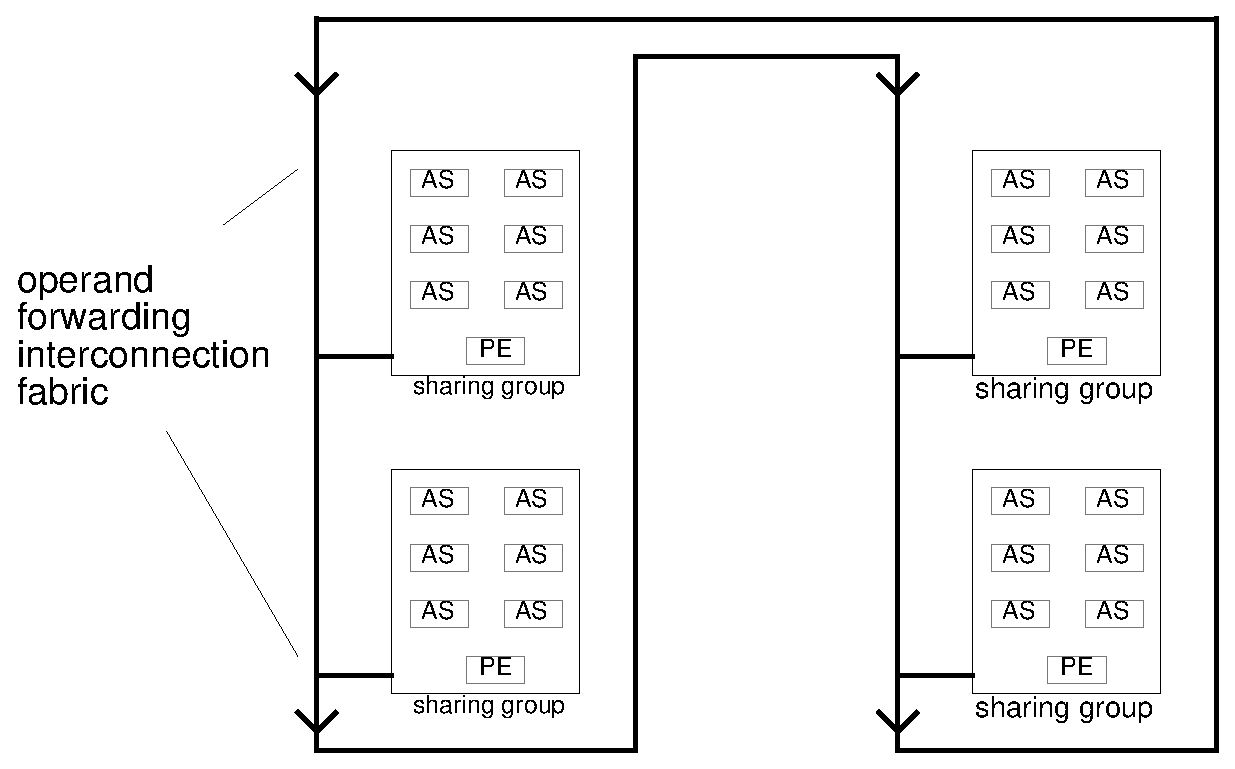
\epsfig{file=window.eps,width=5.0in}
\caption{{\em Execution Window.} Shown are four sharing groups
each with six active stations and one shared processing element.
There are six rows of ASes in each column of the entire arrangement.}
\label{fig:window}
\end{figure}
%
We dispatch instructions to the ASes simultaneously, a column at
a time.  At a maximum, new instructions can be dispatched to a column every
cycle.  Although desirable, this is not always possible since a
corresponding column of ASes would need to be retired at the same rate.
To manage control, register data, and memory
data dependencies, we make extensive use of time tags.

Fortunately, our present model for program execution provides
a very key advantage to exploiting a large and distributed microarchitecture.
Since in-order dispatched instructions 
only need to forward (versus backward) results into the
program-ordered future, there is no real need to provide connectivity
to previously executed instructions 
(previous in program order).  This is the basic
idea of laying out the active stations in columns.  Result operands
from one instruction will flow forward to the next program instructions
that are in the ordered future of the program (whether those
instructions are speculative or not).  
%
%
\subsection{Time Tags and Renaming}
%
A time tag indicates
the position of an instruction in the original 
sequential program order (i.e., in the order that instructions are 
dispatched
to active stations).  
Active stations are labeled with time tags starting
from zero and incrementing up to one minus the total number of
active stations in the microarchitecture.  
A time tag is a small
integer that uniquely identifies a particular active station.
Time tags can be thought of as having two
parts.  Since the active stations are laid out
in columns and rows, time tags can be viewed as having a column
component and a row component.  The column component 
occupies the high order bits of
the time tag integer and the row component occupies the remaining space.

For illustrative purposes, we usually assign time tags, starting with the
value zero,
to active stations starting at the upper left corner of the two
dimensional grid of active stations and proceed to assign incremented
time tags first down the left-most column and continuing down the
next column to its right until all active stations are numbered.

Similarly to the conventional reservation station, operand results
are broadcast forward for use by waiting instructions.
With active stations, all operands that are forwarded after the execution
of an instruction are also tagged with the time tag value of the
active station that generated the updated operand.
This tag will be used by subsequent active stations to determine if
the operand should be {\em snarfed}~\footnote{snarfing entails snooping
address/data buses, and when the desired address value is detected, 
the associated data value is read} 
as an input operand that will trigger
the execution of its loaded instruction.

Essentially all values within the execution
window are tagged with time tags.
Since our microarchitecture can also allow for the concurrent
execution of multiple speculative paths of the current program,
we also introduce a path identifier (path ID).
A path ID 
identifies the current path that an active station 
is executing an instruction for.  
We allow for multiple speculative execution paths to
exist within the execution window (instructions have been
dispatched to ASes) simultaneously.
Not all applicable microarchitectures may uses multiple speculative
execution paths but we plan for that case anyway.
Path IDs are numbered from zero
to one minus the total number of possible paths.
Path IDs are assigned to all operands in the execution window
along with time tags.

The microarchitecture that we have devised requires the
forwarding of three types of operands.  These are register
operands, memory operands, and instruction predicate operands.
Register and memory operands are identical to those of
conventional microarchitectures but the predicate operand is
something that is not as generally used or understood in
existing conventional machines and is therefor described a bit further.
Our predicate operand is
a single bit register that we associate with each instruction and
which is used to predicate its execution.  It is not an architected
register of the ISA ; 
in that case it would be a regular register operand in our microarchitecture
and not what we refer to as a predicate operand at all.
All of these operands are tagged with time tags 
and path IDs that were associated
with the active stations that produced them.
The information 
broadcast from an AS to subsequent
ASes in future program ordered time is referred
to as a {\em transaction}, and generally consists of :
%
\vspace{-0.05in}
\begin{itemize}
\vspace{-0.1in}
\item{the type of the transaction}
\vspace{-0.1in}
\item{a path ID}
\vspace{-0.1in}
\item{the time tag of the originating active station}
\vspace{-0.1in}
\item{the identifier of the architected operand}
\vspace{-0.1in}
\item{the actual data value for this operand}
\vspace{-0.1in}
\end{itemize}   
%
More details on transactions for register, memory, and
predicate forward operations is presented in a later section.
This above information is typical of all transactions that
convey operand values into future program order time.

Figure \ref{fig:source} shows the registers inside an active
station for one of its input operands.  The 
{\em time-tag},
{\em address}, and
{\em value} registers are reloaded with new values on each snarf,
while the
{\em path} and
{\em AS time-tag} are only loaded when an instruction is
dispatched to the active station.
The operand shown is typical for source registers, a source memory
operand, or an instruction execution predicate register.
%
\begin{figure}
\centering
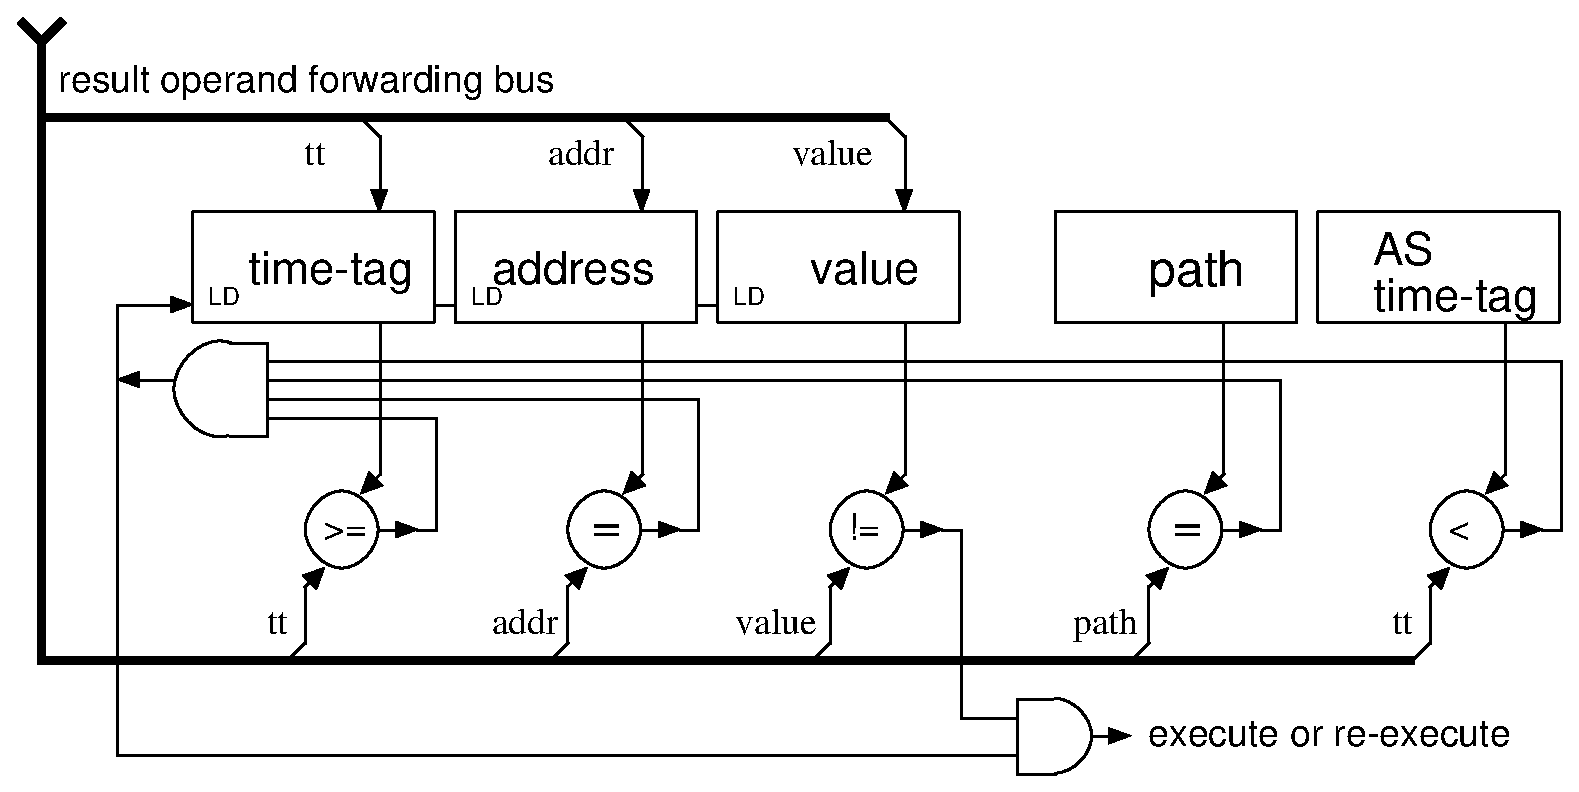
\epsfig{file=source.eps,width=5.0in}
\caption{{\em Active Station Source Operand.} The registers and snooping
operation of one of several possible source operands is shown.
Just one operand forwarding bus is shown being snooped but
typically several operand forwarding buses are snooped simultaneously.}
\label{fig:source}
\end{figure}
%
In the case of a register operand being forwarded, the name of the
operand is the address of the architected register.  For example
if the architected register in question is {\tt r6} then the
name of that operand would be the value 6.  If the operand
being forwarded is a memory operand, then the name of the operand
is simply its address (either a 32-bit address or a 64-bit address
depending on the machine ISA).  If the operand is a predicate,
then the name might be an internally derived value depending on
the predication implementation. 

This scheme effectively eliminates the need for rename registers
or other speculative registers as part of the reorder buffer.
The whole of the microarchitecture thus provides for the full renaming
of all operands, thus avoiding all false dependencies.
There is no need to limit instruction dispatch or to limit speculative
instruction execution due to a limit on the number of non-architected
registers for holding those temporary results.

True flow dependencies are enforced through continuous  
snooping by each active station.  Each active station
will snoop all operands that are broadcast to it.  If the
path ID and the architected name of the operand match any of
its current input operands, the active station then checks
if the time tag value is less than its own assigned time tag,
and greater than or equal to the time tag value of the last
operand that it snarfed, if any.  If the snooped data value is
different than the input operand data value that the active
station already has, a re-execution of the instruction is initiated.
This simple rule will enforce
all proper flow dependencies while allowing for massive
concurrency to occur.
%
%
\subsection{Result Forwarding Buses}
%
There are several choices for a suitable interconnection fabric between
the active stations.  Our fabric uses segmented buses with buffers
between stages; this preserves
scalability and provides reasonable performance (we exploit the fact
that register lifetimes only span 1 or 2 basic blocks).
This paper will not address the
many options that are available.  
A representative interconnection fabric is shown in Figure \ref{fig:window}
connecting all of the sharing groups.
Repeater units that break up the interconnection fabric are not
shown in the figure but are required in an actual implementation
The purpose of the
interconnection fabric is to primarily forward instruction result
operands, tagged with their time tags, 
to those active stations in the program ordered future (those
active stations with higher valued time tags).  This means that one
basic requirement of the interconnection fabric is that it must be able
to transport operand results from any active station in a column to
those active stations lower in the same column and then to the remaining
active stations to the right of the current column starting again at
the top of the next column to the right.  So regardless of the number
and types of connections for interconnecting buses, the buses must
allow for the flow of operands from top left-most active station in the
grid, down the left-most columns of ASes, up to the top of the next and
repeating for all columns.

It must be noted at this point that operand result forwarding
bus connectivity is also needed (in a seemless way) from the bottom
right-most active station to the top left-most active station.
This is needed because assignment of time tags (as discussed so far)
is not going to remain static during the actual operation of the machine.
As columns of ASes retire and new instructions are dispatched to
free columns,
all of the time tags in the execution window are decremented by
an amount equal to the numbers of ASes in a column.  This corresponds
to decrementing the column part of each time tag in the whole of the
execution window by one.  The decrementing of all time tags
occurs when a column of instructions (in the ASes) is retired.
Newly dispatched instructions will take on
time tag values corresponding to the right-most 
column of ASes.  The oldest column becomes the 
newest column.  Since columns are connected by a toroidal network in the
execution window, this corresponds to a sort of logical shift
of the columns along the ring formed by the interconnection
network.  This operation of the machine is thus termed a \textit{shift}
and is associated with both a new column of instructions being dispatched
as well as the decrementing of the column part of all of the time tags
in the machine.
%
%
\subsection{Operand Forwarding Strategies and Bus Transactions}
%
Although we have so far described the operand forwarding mechanism
in simple terms as being the broadcasting of it 
to those ASes with higher valued 
time tags, there are some additional details that need to be
addressed for a correctly working forwarding solution.
These details also differ depending on whether operands for
register, memory, or predicates need to be forwarded.
There are many possible strategies for forwarding of operands
(and of operands of differing types). 
We now briefly outline three such strategies.
One of these is suitable for registers.
Another is suitable for registers or memory operands.
The third is oriented for the forwarding of predicates.
These three strategies are termed \textit{relay forwarding},
\textit{nullify forwarding}, and \textit{predicate forwarding}
respectively.
In general, each forwarding strategy employs bus transactions
of one or more types to implement its complete forwarding solution.
The particulars of these transactions are described for each
of the forwarding strategies.
%
%
\subsubsection{Relay Forwarding}
%
This forwarding strategy is quite simple but is also entirely
adequate for the forwarding of register operands.
In this strategy, when a new register operand needs to be forwarded
from an active station, the standard operand information, as 
previously described
in a general, is packaged up into what is termed
a \textit{register store} transaction.
This transaction type consists of :
%
\vspace{-0.05in}
\begin{itemize}
\vspace{-0.1in}
\item{a transaction ID of \textit{register store}}
\vspace{-0.1in}
\item{the path ID on which this instruction is executing}
\vspace{-0.1in}
\item{the time tag of the originating active station}
\vspace{-0.1in}
\item{the register address}
\vspace{-0.1in}
\item{the value of the register}
\vspace{-0.1in}
\end{itemize}   
%
A request is made to arbitrate for an outgoing forwarding bus
and this transaction is placed on the bus when it becomes available.

When the instruction associated with an active station gets
a new input operand, it will re-execute producing a new
output operand.  In this forwarding strategy, the new output
operand is both stored locally within the active station itself
and is sent out on the outgoing forwarding buses
to subsequent (higher time-tag valued) active stations.
Previous values of the instruction's output operand is also
snooped as if it was an input operand and is also stored locally
within the active station.
It should also be noted that if the enabling execution predicate
for the current instruction changes, either from being enabled
to disabled or visa versa, a new output operand is forwarded.
If the instruction predicate changes from disabled to enabled,
the output operand that was computed by the instruction os
forwarded.  If the instruction predicate changes from enabled
to disabled, the previous value of the output operand (before being
changed due to the instruction execution) is forwarded.
That previous value is available to the active station because
it gets snooped as if it was an additional input.
Newly forwarded operands will always superseded and previously
forwarded operands.
With this strategy, instructions that are located in the program
ordered future will eventually always get the correct
value that will end up being the committed value if the
current instruction ends up being committed itself (ends
up being predicated to execute).
This is an elegant forwarding strategy and
the simplest of the forwarding strategies investigated so far, and
is a reasonable choice for the handling register operands.
The inclusion of the time tag in the transaction is the
key element that allows for the correct ordering of
dependencies in the committed program.
%
\subsubsection{Nullify Forwarding}
%
There are limitations to the applicability of the previously
discussed forwarding strategy (relay forwarding).
That strategy depends upon the fact that the address of the
architected operand does not change during the life time of
the instruction while it is in an active stations.
For example, the architected addresses for register operands
do not change for instructions.  If the instruction takes
as an input operand a register \textit{r6} for example,
the address of the operand never changes for this particular
instruction (it stays \textit{6}).
This property is not generally true of memory operands.
The difficulty with memory operands is that many memory
related instructions determine the address of a memory operand
value from an input register operand of the same instruction.
Since we allow for instructions to execute and re-execute
on entirely speculative operand values, the values of
input register operands can be of essentially any value
(including a wilding incorrect value) and thus the
address of a memory operand can also change during the during
that the instruction is in flight within the active station.
This presents a problem for the correct enforcement of
memory operands, and dependencies among them, in the entire program.
If we examine the case of a memory store instruction,
when it
re-executes acquiring a new memory store value, the address of that
memory store may also have changed !  
We cannot simply forward that new memory operand (address and value)
as with the relay forwarding strategy above.  The reason is
that we would not be superseding the previous memory operand
that we forwarded previously that quite likely had a different
architected address.  Rather, we need some way to cancel the effect of
any previously forwarded memory operands.
This present forwarding strategy does just that.

In this strategy, memory operands that need to be forwarded
employ a similar transaction as above for registers (described
in the context of relay forwarding) but would instead have
a transaction ID of \textit{memory store} and would
include the memory operand address and its value (along with the
path and time-tag information).
However, when an instruction either re-executes or
its enabling predicate changes to being disabled, a different
type of forwarding transaction is sent out.
This new type of transaction is termed a \textit{nullify transaction}
and has the property of nullifying the effect of a previous
store transaction to the same architected operand address.
This transaction type consists of :
%
\vspace{-0.05in}
\begin{itemize}
\vspace{-0.1in}
\item{a transaction ID of \textit{memory nullify}}
\vspace{-0.1in}
\item{the path ID on which this instruction is executing}
\vspace{-0.1in}
\item{the time tag of the originating active station}
\vspace{-0.1in}
\item{the memory operand address}
\vspace{-0.1in}
\item{the value of the memory operand}
\vspace{-0.1in}
\end{itemize}   
%
When this transaction is snooped by subsequent ASes,
for those ASes that have a memory operand as an input
(that would be for instructions that load memory values in
one way or another)
a search is made for a match of an existing memory
operand as usual but if a match is detected,
the time-tag of that particular memory operand is set to
a state such that any future \textit{memory store} transaction,
regardless of its time-tag value, will be accepted.
Further, on reception of this \textit{memory nullify} transaction,
a request is sent backwards in program order for a memory
operand with the desired memory address.
The transaction that represents a request for a memory
operand would consist of :
%
\vspace{-0.05in}
\begin{itemize}
\vspace{-0.1in}
\item{a transaction ID of \textit{memory request}}
\vspace{-0.1in}
\item{the path ID on which this instruction is executing}
\vspace{-0.1in}
\item{the time tag of the originating active station}
\vspace{-0.1in}
\item{the memory operand address}
\vspace{-0.1in}
\end{itemize}   
%
Of course, the memory address for the operand desired
needs to be in the transaction but it is not as obvious why
the originating AS's time tag is also included.  In some
interconnection fabrics, the time tag is included in backwarding
requests to limit the scope of the travel of the transaction
through the execution window.  This same scope-limiting function
is usually performed for forward going transactions as well.
When the request is sent backwards in program order, previous
ASes or the memory unit itself will eventually snoop
the request and respond with another \textit{memory store}
transaction.
As discussed, this forwarding strategy is very useful for memory
operands but it can also be used for register operands with
appropriate changes to the applicable transaction elements.
Again, the inclusion of a time tag value is what allows
for proper operand dependencies (whatever they may be for
any particular forwarding strategy) in the committed program.
%
\subsubsection{Predicate Forwarding}
%
There are several ways in which instructions can be predicated
in the microarchitecture.  
These predication mechanisms are not discussed in
this paper but two such mechanisms are can be found in
documents by Uht et al ~\cite{Uht01} and Morano ~\cite{Morano02}.
For microarchitectures that predicate all program instructions
within the microarchitecture itself (not visible at the ISA
level of abstraction), predicate register values are essentially
operands that need to be computed, evaluated, and forwarded
much like register or memory operands.
Each instruction computes its own enabling predicate by
snooping for and snarfing predicate operands that are forwarded
to it from previous instructions from the program ordered past.
Depending on the particular predication mechanism used,
relay forwarding (described above) may be a suitable (if not good) choice 
for handling the forwarding of predicate operands.
However, some predication mechanisms need additional transaction
types (besides a base store transaction) to communicate.
The predication mechanism described by Morano in ~/cite{Morano02}
requires three transaction to fully implement.
That mechanism was employed for the data generated (presented in
a following section), and the transactions for that mechanism
are briefly described here.

This predication strategy requires two store-type transactions
rather than just one.  These two transactions are similar
to other operand store transactions (like for register or memory
operands)
but one of these holds two values rather than just one.
The first of these is the \textit{region predicate store}
transaction and consists of :
%
\vspace{-0.05in}
\begin{itemize}
\vspace{-0.1in}
\item{a transaction ID of \textit{region predicate store}}
\vspace{-0.1in}
\item{the path ID on which this instruction is executing}
\vspace{-0.1in}
\item{the time tag of the originating active station}
\vspace{-0.1in}
\item{the region predicate value}
\vspace{-0.1in}
\end{itemize}   
%
This transaction is very analogous to a register or memory
store but instead is used to forward a single bit value (the
current \textit{region predicate} for instructions following the
AS that forwarded the transaction).  A region predicate
is a single bit that determines the execution status
(enabled or disabled) for instruction that lie beyond the
not-taken output path of a conditional branch.
This particular transaction could be forwarded by either
a conditional branch or by a an instruction that was not
a control-flow-change instruction.  In the
case of a non-control-flow-change instruction, the only
predicate value that makes sense is the same as its
own enabling predicate and so only one value need
be forwarded.

In the case of a conditional branch instruction,
there are two possible output predicates that can be in
view.  One is for the not-taken output path from the branch.
The other is for the taken output path.
In order to forward both values for those instructions
in program ordered future, the other store transaction
type (mentioned previously) us used.
This transaction consists of :
%
\vspace{-0.05in}
\begin{itemize}
\vspace{-0.1in}
\item{a transaction ID of \textit{branch target predicate store}}
\vspace{-0.1in}
\item{the path ID on which this instruction is executing}
\vspace{-0.1in}
\item{the time tag of the originating active station}
\vspace{-0.1in}
\item{the branch target instruction address}
\vspace{-0.1in}
\item{the region predicate value}
\vspace{-0.1in}
\item{the branch target predicate value}
\vspace{-0.1in}
\end{itemize}   
%
This is identical to the previous \textit{region predicate store}
transaction but also includes the instruction address
for the target of the conditional branch (the \textit{taken} address)
and the single bit predicate
governing the execution status for instructions
following the target of the conditional branch in program ordered
future.

Finally, for the predication mechanism employed in the present
work, a third transaction is used to invalidate a previously
forwarded branch target predicate.  This transaction is
a \textit{branch target invalidation} and consists of :
%
\vspace{-0.05in}
\begin{itemize}
\vspace{-0.1in}
\item{a transaction ID of \textit{branch target invalidation}}
\vspace{-0.1in}
\item{the path ID on which this instruction is executing}
\vspace{-0.1in}
\item{the time tag of the originating active station}
\vspace{-0.1in}
\item{the branch target instruction address}
\vspace{-0.1in}
\item{the time tag of the branch target predicate to be invalidated}
\vspace{-0.1in}
\end{itemize}   
%
This is similar to other such invalidation transactions in
that when it is snooped by ASes in the program ordered future,
a search is made for some state (in this case some predicate
register state) that matches the given transaction criteria.
The inclusion of the second time tag in this transaction allows
for certain efficiencies that are particular to the predication
mechanism described.

For predicate forwarding, as we have seen for register and
memory forwarding, time tags play the vital role in
identifying and preserving the ordering of all operands.
In many ways, all operands (whether they be registers, memory,
or execution predicates) require the use of time tags to
determine the relative ordering of events in a microarchitecture
that otherwise lets all instructions execute and re-execute
wildly out of order in real time with respect to each other.
%
%
\section{Simulation Results}
%
Using an execution-driven simulator, we ran
SpecInt-2000 and SpecInt-95 programs on our
time-tagged microarchitecture.  
Our goal here was to evaluate
the instruction per clock (IPC) that was possible using
the microarchitecture.
Ten benchmark programs were used
in all.  
Seven programs are from the SpecInt-2000 suite and
three are from the SpecInt-95 suite.  
These programs were
chosen in order to get a variety of execution behaviors.
The microarchitecture simulated supports 
the MIPS-1 ISA (big endian), with some MIPS-2
instructions also supported in order to accommodate code residing in
the SGI system libraries which use them.
All programs were compiled using the vendor SGI compiler on
the SGI IRIX 6.4 operating system.
Programs were compiled with
standard optimization ({\tt -O}) for primarily the MIPS-1 ISA ({\tt -mips1}).
The first 600 million instructions of all programs were
executed.  Data were only gathered after the execution of
the first 100 million instructions (a total of 500 million).
The default features of the machine simulated are
given in Table \ref{tab:params}.
%
\begin{table}
\begin{center}
\caption{{\em General machine characteristics.}
These machine parameters are used for all simulations as
the default except where one of these parameters may be varied.}
\label{tab:params}
\begin{tabular}{|l|l|}
\hline 
L0 cache size&32 words\\
\hline 
L1 I/D cache access latency&1 clock\\
\hline
L1 I/D cache size&64 KBytes\\
\hline
L1 I/D block size&32 bytes\\
\hline
L1 I/D organization&2-way set associative\\
\hline
L2 cache access latency&10 clocks\\
\hline
L2 cache size&2 MBytes\\
\hline
L2 block size&32 bytes\\
\hline
L2 organization&direct mapped\\
\hline
main memory access latency&100 clocks\\
\hline
forwarding unit minimum latency (all)&1 clock\\
\hline
forwarding-bus latency (all)&1 clock\\
\hline
number of register forwarding buses&2\\
\hline
number of predicate forwarding buses&2\\
\hline
number of memory buses&1\\
\hline
branch predictor&PAg\\
\cline{2-2}
 & 1024 PBHT entries\\
\cline{2-2}
 & 4096 GPHT entries\\
\cline{2-2}
 & saturating 2-bit counter\\
\hline
\end{tabular}
\end{center}
\end{table}
%
The data in Table \ref{tab:ipc1} contains IPC 
results for a range of machine sizes.
All machines simulated also contained two forwarding buses for
register operands, two forwarding buses for predicates, and
one forwarding bus for memory operands.
All forwarding buses incur a bus transfer delay of 1 clock.
Further, each forwarding unit encountered (different for different
machine sizes) has a minimum latency of 1 clock.
All simulated machines, regardless of size, have forwarding buses
that span eight sharing groups.  This illustrates how the bus
length can be constant with respect to the machine size thus allowing
for physical scalability of the machine.
Machine sizes are basically characterized by
Each of the machine configurations in Table \ref{tab:ipc1} consists of three
numbers that give the rows of sharing groups, the number
of active station rows per sharing group, and the total number of 
columns respectively.  The number of sharing group rows times the
number of active stations per sharing group is the total number of
active station rows in a configuration.  The product of all three
numbers gives the total number of ASes in the machine and therefor
the number of instructions that may be in flight 
simultaneously
(having
possibly speculatively executed already).
%
\begin{table}
\begin{center}
\caption{{\em Benchmark IPC results for various machine sizes.}
Different machine sizes are characterized by their
geometries consisting of the three-number entries along the
top of the table: SG rows per column, AS rows per SG, and
SG columns.}
\label{tab:ipc1}
\begin{tabular}{|l|c|c|c|c|c|c|c|c|}
\hline 
config&
8-4-8&8-4-12&12-4-8&8-8-8&8-12-8&8-16-8&16-8-8&32-8-8\\
\hline
\hline 
bzip2&4.1&4.1&4.3&4.9&5.2&5.5&4.9&5.1\\
\hline 
compress&4.1&4.3&4.3&4.7&4.8&4.8&4.8&4.9\\
\hline 
crafty&3.7&3.8&3.8&4.1&4.2&4.1&4.1&4.4\\
\hline 
gcc&3.1&3.1&3.1&3.3&3.3&3.3&3.4&3.6\\
\hline 
go&4.1&4.6&4.7&5.1&5.5&5.4&5.3&6.0\\
\hline 
gzip&4.8&5.0&5.2&6.1&6.5&6.4&6.4&6.5\\
\hline 
ijpeg&6.2&7.2&7.8&9.5&12.3&13.1&12.0&12.3\\
\hline 
mcf&3.5&3.5&3.6&4.3&4.7&5.3&4.5&5.0\\
\hline 
parser&3.5&3.7&3.5&3.9&4.0&3.9&3.9&4.4\\
\hline 
vortex&4.2&4.4&4.7&4.8&4.9&4.6&4.9&5.1\\
\hline 
\hline 
H-MEAN&3.8&4.2&4.3&4.7&4.9&5.06&4.9&5.2\\
\hline
\end{tabular}
\end{center}
\end{table}
%
Generally, as the number of active stations increases,
the resulting IPCs also increase, but there are diminishing returns.
A significant IPC gain is achieved, for example, when increasing the
size of the machine from the 8-4-8 geometry (256 ASes) to the 8-8-8 geometry
(512 ASs).  This is an increase in IPC of approximately 17.8\% on the
harmonic mean across all benchmarks.  However, doubling the number
of active stations again (the number of instructions in flight
in the e-window simultaneously) to 1024 with the 16-8-8 machine geometry,
the harmonic mean IPC only increases by about 3.4\%.  Even an
alternative geometry (the 8-16-8 geometry) also having 1024 ASs
gives a harmonic mean IPC of 4.96, an increase of approximately 5.6\%
over the 8-8-8 geometry.
Comparing the 8-16-8 geometry with the 16-8-8 geometry (both having
1024 ASes), the results from each are fairly similar with the
8-16-8 geometry edging out the 16-8-8 when all benchmarks are
considered.  However, for some benchmarks (like GCC and VORTEX)
the IPC are lower with the 8-16-8 geometry.  This suggests that
there is little benefit in just increasing the number of active station
rows per sharing group after some point (16 in the present) case
since contention for the single common processing logic starts
to limit performance.
With the current state of this microarchitecture research,
the best tradeoff of resources and IPC results would appear
to be with the machine geometry of 8-8-8.  This consists of 512
ASs and the associated bus interconnects between them. 
Without the use of time tags as an operand dependency enforcing
mechanism, it is not clear how this arrangement could otherwise be 
implemented
in current or near-term process technologies due to interconnection
and contention problems that would arise.

A better look at the potential of this microarchitecture is
presented by the IPC data in Table \ref{tab:ipc2}.
Some of the configurations presented previously, 
in Table \ref{tab:ipc1},
are repeated but this time they were executed with a relaxed
assumption about the branch prediction accuracy guiding the
fetching and dispatching of instructions into the e-window.
In this data set, 100\% branch prediction accuracy was
assumed in an attempt to see what might be possible with this
general microarchitectural approach as research continues to
make possible i-fetch improvements.
%
\begin{table}
\begin{center}
\caption{{\em Benchmark IPC results for various machine sizes
when assuming 100\% branch prediction accuracy guiding i-fetch.}
Different machine sizes are characterized by their
geometries consisting of the three-number entries along the
top of the table: SG rows per column, AS rows per SG, and
SG columns.}
\label{tab:ipc2}
\begin{tabular}{|l|c|c|c|c|}
\hline 
config&
8-4-8&8-8-8&16-8-8&32-8-8\\
\hline
\hline 
bzip2&9.0&12.4&15.5&16.3\\
\hline 
compress&8.1&12.2&16.2&17.6\\
\hline 
crafty&6.1&9.3&14.7&21.7\\
\hline 
gcc&7.1&12.3&17.3&21.2\\
\hline 
go&9.0&12.3&17.3&21.2\\
\hline 
gzip&7.6&10.0&11.2&11.5\\
\hline 
ijpeg&9.2&14.4&18.7&20.2\\
\hline 
mcf&6.1&8.2&10.1&12.0\\
\hline 
parser&7.3&10.9&14.6&17.0\\
\hline 
vortex&6.4&10.1&15.2&21.7\\
\hline 
\hline 
H-MEAN&7.3&10.8&13.3&16.9\\
\hline
\end{tabular}
\end{center}
\end{table}
%
In this IPC data, results continue to improve up through the
32-8-8 machine geometry.
Any realization of a machine with this number of speculative
instructions in flight (2048 in this case) is clearly not
feasible given current operand enforcement methods like
a reorder buffer.  Contention for access to it would be too great
given current and foreseeable silicon limitations.
%
%
\section{Related Approaches}
%
The Warp Engine~\cite{Cleary95} used time tags; however their implementation
is cumbersome, utilizing floating point numbers and machine wide parameter
updating.  The Metaflow Architecture discusses the 
idea of {\em delayed scheduling}
to obtain moderate gains in ILP~\cite{Pop}.

By developing a microarchitecture based around active stations
and the use of time tags to coordinate and enforce correct program
order, we eliminate the need for the severe contention present 
on either register scoreboards \cite{Thornton64} 
or the architected register files associated
with the use of reservation stations~\cite{Anderson67}.  

In those microarchitectures
that perform speculative execution, there is also
the need to access the reorder buffer, which becomes quite problematic
as the number of instructions being speculatively executed concurrently
grows~\cite{Palacharla}.  Whether speculative instruction operand
results are stored in data registers within the reorder buffer or if the
results are stored in extra physical registers that hold both architected
and temporary values, the contention for the centralized resource is
the same.  In our microarchitecture, the set of active
stations form a giant reorder buffer.  The registers that
make up a reorder buffer in a conventional microarchitecture are
not eliminated entirely in the sense that we store the same speculative
information in a distributed way in each active station.  Similarly,
although the need for centralized rename registers is eliminated,
we are effectively storing the rename registers along with the
decoded instructions inside each active station.  
%
%
\section{Summary}
%
We have presented a new microarchitecture
that uses time tags to coordinate and enforce
program order on a very large scale and with a large degree
of rampart out-of-order execution.
The scheme presented allows for the execution of instructions
with entirely speculated source operands, and it properly
handles cases when these operands are speculative register,
memory, or execution predicate values.
The use of time tags allows for a degree of out-of-order
execution that is not easily enforceable using any other
mechanism due to either routing congestion or access contention
problems.
The use of the time tags therefor allow for scalability of our 
microarchitecture
to sizes that can allow for hundreds of instructions (or more) to execute
concurrently.
Our results indicate that this general approach appears to be quite
promising as compared with the existing more conventional microarchitectural
approaches.  
Some work on much larger machine configurations has already
suggested that achieving IPC numbers in the 10s on general integer
sequentially-oriented program codes is possible.
%
\bibliographystyle{latex8}
\bibliography{timetags}
%
\end{document}
%
%
%
%
